\documentclass[12pt,a4paper]{standalone}
\usepackage[utf8]{inputenc}
\usepackage{amsmath}
\usepackage{amsfonts}
\usepackage{amssymb}
\usepackage{xparse}
\usepackage{physics}
\usepackage{tikz}
\usetikzlibrary{calc}
\author{Disha J. Kuzhively}
\begin{document}
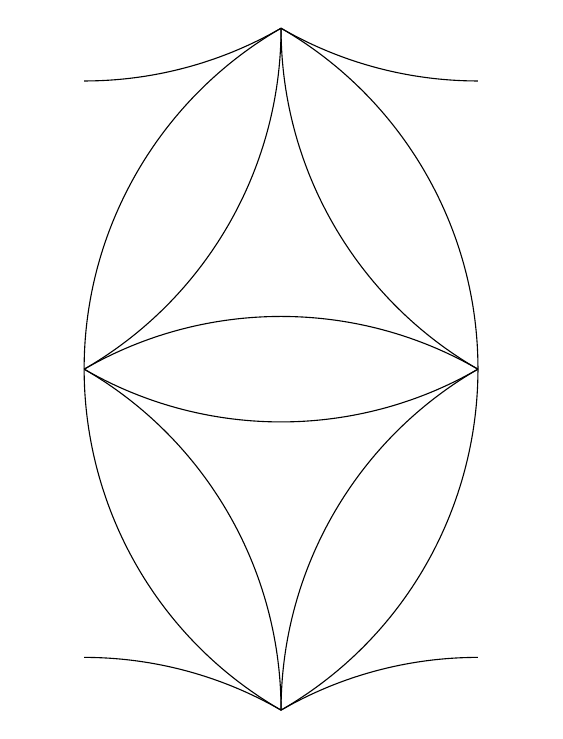
\begin{tikzpicture}

\draw (60:5) arc [start angle=60, end angle=120, radius=5];
\draw (60:5) arc [start angle=-60, end angle=-120, radius=5];
\draw (0,0) arc [start angle=-60, end angle=60, radius=5];
\draw (0,0) arc [start angle=240, end angle=120, radius=5];
\draw (0,0) arc [start angle=180, end angle=120, radius=5];
\draw (0,0) arc [start angle=0, end angle=60, radius=5];
\draw (60:5) arc [start angle=240, end angle=180, radius=5];
\draw (120:5) arc [start angle=-60, end angle=0, radius=5];
\draw (0,0) arc [start angle=120, end angle=90, radius=5];
\draw (0,0) arc [start angle=60, end angle=90, radius=5];
\draw (90:{sqrt(75)}) arc [start angle=240, end angle=270, radius=5];
\draw (90:{sqrt(75)}) arc [start angle=300, end angle=270, radius=5];
\end{tikzpicture}
\end{document}